% !TeX spellcheck = en_US
\addscenariosection{1}{Clash Scenario}{The Obelisk}{\images/obelisk.png}

\begin{multicols*}{2}

\textbf{Author:} Pinkerton, biigrick, LAAMAKALA

\textbf{Source:} \href{<https://discord.com/channels/740870068178649108/1232319328049954826>}{Archon Studio's Discord}

\textit{The map is torn, the path unclear — but the obelisks call. Rally your armies, master your magic, and stake your claim before another hero takes the prize.}  % no-check-caps

\subsection*{\MakeUppercase{Scenario Length}}
This Scenario plays out over 8-10 Rounds.

\subsection*{\MakeUppercase{Player Setup}}
\textbf{Player Count:} 2-6 FFA or Alliance

Choose starting \textbf{Resources, Income, Units} and \textbf{Town Buildings} from any Scenario.

\textbf{Map Tile Pool:} Each player takes 2 random Far (II--III) Map Tiles.

\subsection*{\MakeUppercase{Map Setup}}
Take the following Map Tiles and arrange them as shown in the Scenario map layout ($P$ stands for the number of players):

\begin{itemize}
  \item P × Starting (I) Map Tiles
  \item 7 × Near (IV-V) Map Tiles (4 with Obelisks)
\end{itemize}

\subsection*{\MakeUppercase{Victory Condition}}
The game ends when one or more Victory Condition is met: Player who
\begin{itemize}
  \item starts their turn controlling two or more Obelisks or
  \item controls two or more Obelisks at the end of Round 10,
\end{itemize}
wins the game. If none of the Victory Conditions are met or in the case of a tie, the Player controlling the Center Obelisk wins the game.

\subsection*{\MakeUppercase{Timed Events}}
\textbf{\nth{3}, \nth{6} and \nth{8} Round:}
\begin{itemize}
  \item Remove all Black Cubes from the Map.
\end{itemize}

\subsection*{\MakeUppercase{Additional Rules}}
\begin{itemize}
  \item \textbf{Obelisk:} If you are first Player to flag the Obelisk, choose one adjacent Visitable Field and gain its reward.
  \item Any Hero starting their turn on a Far Tile gains +1 \svgeven{movement}.
  \item You may add any Additional Rules from other Scenarios.
\end{itemize}

\begin{center}
  \vfill
  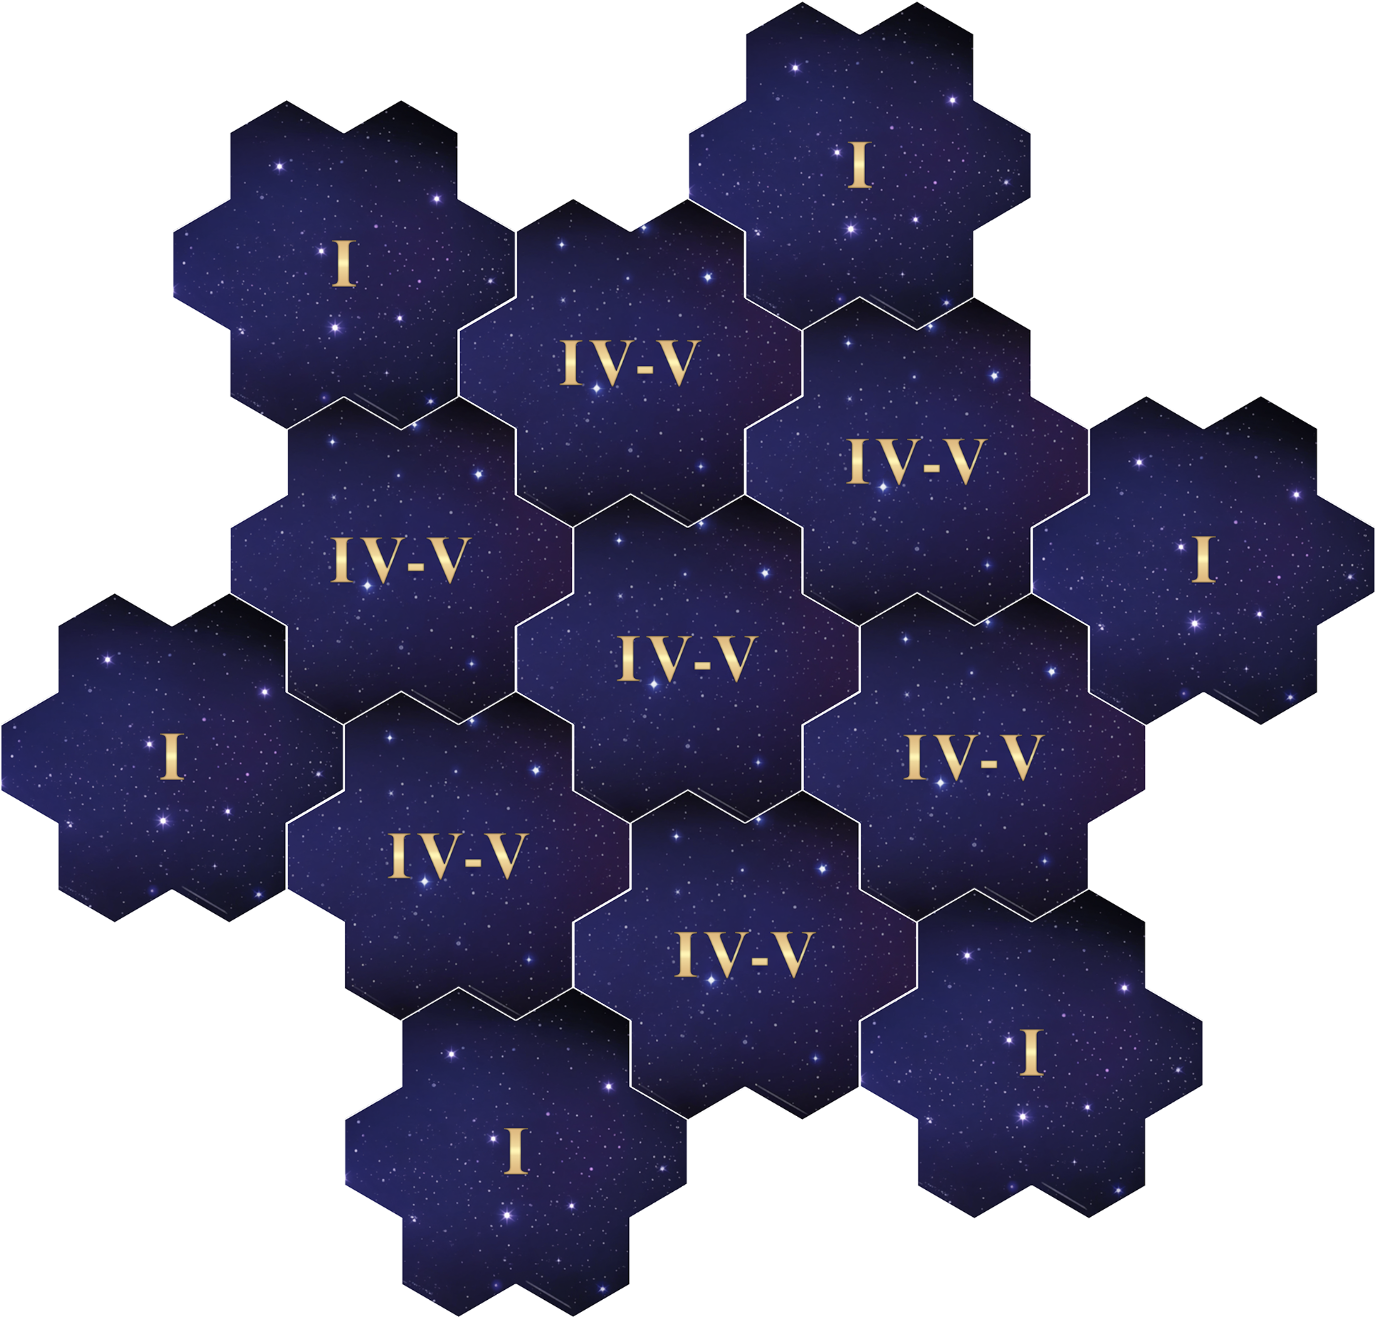
\includegraphics[width=1.0\linewidth]{\maps/obelisk.png}
  \captionof{figure}{\textbf{SCENARIO MAP LAYOUT}}
  \vfill
\end{center}

\end{multicols*}

